\documentclass[10pt]{article}
\usepackage{fullpage}
\usepackage[pdftex]{graphicx}
\usepackage{rotating}
\usepackage{multirow}
\usepackage{subfigure}
\usepackage{url}
\usepackage{amsmath}
\usepackage{amssymb}
\usepackage{wasysym}
\usepackage{algorithm}
\usepackage{algpseudocode}

\newcommand{\etal}{\emph{et al.}}

\begin{document}
\title{K Nearest Neighbour Search Using Space-filling Curves}
\author{Camara Lerner \hspace{2cm} Christopher Rabl \\
  Department of Mathematics and Computer Science \\
  University of Lethbridge, Canada}

\maketitle

\section{Introduction}

All methods of calculating K-Nearest Neighbours (KNN) are marred by the ``curse of dimensionality'' \cite{Bellman:2003}. Even though it is not an NP-Complete problem, it is still difficult to calculate KNN in high dimensions. Approaches such as spatially ordered trees (such as quadtrees and $kd$-trees) and space-filling curves have been applied to this problem in order to solve it more quickly than the naive approach (calculating a distance matrix between each point and choosing the smallest $k$ entries from the row corresponding to the query point $q$).

\section{Method of Dahl and Wootters}

Contrary to the project proposal, the authors decided against exploring the approach of Dahl and Wootters \cite{Dahl:2008} due to a significant lack of implementation specificity: many important details were completely omitted from the paper and could not be extrapolated based on the context of the statements in which they appeared. Instead, a variant of method by Connor and Kumar \cite{Connor:2010} was chosen, since comparing and contrasting the neighbourhood-preserving properties of each space-filling curve turned out to be a more fruitful and unique comparison.

\section{Space-Filling Curves}



\section{Morton Curve}

\begin{algorithm}
  \caption{COMPARE(point ${\bf p}$, point ${\bf q}$)}
  \label{compare}
  \begin{algorithmic}[1]
    \State $x \leftarrow 0, dim \leftarrow 0$
    \ForAll{j=0 to d}
    \State $y \leftarrow \text{FirstMSB}(p_{[j]}, q_{[j]})$
    \If{$x < y$}
    \State $x \leftarrow y, dim \leftarrow j$
    \EndIf 
    \EndFor \\
    \Return $p_{[dim]} < q_{[dim]}$
  \end{algorithmic}
\end{algorithm}

\begin{algorithm}
  \caption{FirstMSB(double $a$, double $b$)}
  \label{first-msb}
  \begin{algorithmic}[1]
    \State $w \leftarrow x < y \text{ and } x < (x \mathrel{\&} y)$ \\
    \Return $w$
  \end{algorithmic}
\end{algorithm}

\begin{algorithm}
  \caption{KNN Graph Construction Algorithm}
  \label{knn-graph-alg}
  \begin{algorithmic}[1]
    \Require $\text{Morton order comparison operator: } < 
    \text{ and Hilbert order compare operator: } <$
    \Ensure $A_i \text{ contains } k \text{ nearest neighbors of } p_i \text{ in } P \text{.}$
    \State $P \leftarrow \text{QuickSort}(P, <)$
    \ForAll{$p_i$ in $P$}
    \State $A_i \leftarrow \text{SET-KNN}(p_i, \{p_{i-k}, \dots, p_{i+k} \})$
    \If{$\text{SHIFT}(p_i, \lceil \text{SET-RAD}(A_i) \rceil) < p_{i+k}$}
    \State $upper \leftarrow i$
    \Else
    \State $I \leftarrow 1$
    \While{$\text{SHIFT}(p_i, \lceil \text{SET-RAD}(A_i) \rceil) < p_{i+2^I}$}
    \State $++I$
    \EndWhile
    \State $upper \leftarrow \text{min}(i+2^I, n)$
    \EndIf
    \If{$\text{SHIFT}(p_i, - \lceil \text{SET-RAD}(A_i) \rceil) > p_{i-k}$}
    \State $lower \leftarrow i$
    \Else
    \State $I \leftarrow 1$
    \While{$\text{SHIFT}(p_i, - \lceil \text{SET-RAD}(A_i) \rceil)$}
    \State $++I$
    \EndWhile
    \State $lower \leftarrow \text{max}(i-2^I, 1)$
    \EndIf
    \If{$lower \not= upper$}
    \State $A_i \leftarrow \text{CSEARCH}(p_i, lower, upper)$
    \EndIf
    \EndFor \\
    \Return $A_i$
  \end{algorithmic}
\end{algorithm}

\begin{algorithm}
  \caption{CSEARCH(point $p_i$, int $lo$, int $hi$)}
  \label{csearch}
  \begin{algorithmic}[1]
    \If{$(hi - lo) < v $}
    \State $A_i \leftarrow \text{SET-KNN}(p_i, A_i \cup \{ p_{lo} \dots p_{hi} \})$
    \Return $A_i$
    \EndIf
    \State $mid \leftarrow (hi+lo)/2$
    \State $A_i \leftarrow \text{SET-KNN}(p_i, A_i \cup p_{mid})$
    \If{$\text{DIST}(p_i, \text{CIRCLE}(p_{lo}, p_{hi})) \ge \text{SET-RAD}(A_i)$} 
    \Return $A_i$
    \EndIf
    \If{$p_i < p_{mid}$}
    \State $A_i \leftarrow \text{CSEARCH}(p_i, lo, mid-1)$
    \If{$p_{mid} < \text{SHIFT}(p_i, \lceil \text{SET-RAD}(A_i) \rceil)$}
    \State $A_i \leftarrow \text{CSEARCH}(p_i, mid+1, hi)$
    \EndIf
    \Else
    \State $A_i \leftarrow \text{CSEARCH}(p_i, mid+1, hi)$
    \If{$\text{SHIFT}(p_i, - \lceil \text{SET-RAD}(A_i) \rceil) < p_{mid}$}
    \State $A_i \leftarrow \text{CSEARCH}(p_i, low, mid - 1)$
    \EndIf
    \EndIf \\
    \Return $A_i$
    
  \end{algorithmic}
\end{algorithm}


\section{Hilbert Curve}

The Hilbert Curve is a space-filling curve that is based on a generalization of Gray codes in $d$ dimensions. The curve is defined based on the amount of space the curve fills. The space that the curve fills can be in any dimensionally space $(n)$ with the length of each dimension filled equal to $2^m$. This means that for each point in the curve the maximum bit size for each dimension is $(m)$. The algorithm used is adapted from~\cite{Hamilton:2006}. \\

The curve labels the points from $0$ to $2^{m*n} - 1$ in the order that the curve visits each point. The Hilbert Curve considered here will start in the bottom left hand corner and finishes in the upper left corner. \\

With Hilbert curves that which uses only one bit called the unit Hilbert curve, is reflected and rotated and moved around to fill the space of the larger Hilbert Curve, and then these unit Hilbert curves are connected to make the overall Hilbert curve. The only constraint on the unit Hilbert curves is that the start and end points must match up with their neighbouring unit Hilbert curves. The same idea is done with gray code, but they  can only be reflected and reversed. These facts are used to inverse the operation of and get the point from the index in the list for both gray code and Hilbert indexing. Hilbert curves also can use information from gray code in determining the changes to the unit Hilbert curve.
 

\flushleft
Formula for Gray Code is in~\ref{gray-code}.
\begin{equation}
  \label{gray-code}
  gc(i) = i \oplus \left( i \gg 1 \right) 
\end{equation}

\begin{algorithm}
  \caption{The algorithm for calculating the Gray Code Inverse $(gc^{-1}(g))$ of $g \in \mathbb{N}$, calculates the $i \in \mathbb{N}$ such that $gc\left( i \right) = g $ }
  \label{gray-code-inverse}
  \begin{algorithmic}[1]
    \Require $g \in \mathbb{N}$ 
    \State $ m \leftarrow \text{ number of bits to represent } g$ 
    \State $ \left( i, j \right) \leftarrow \left( g, 1 \right) $ 
    \While{$ j < m $ }
    \State $ i \leftarrow i \oplus \left( g \gg j \right)$ 
    \State $ j \leftarrow j + 1$ 
    \EndWhile \\
    \Return $i$ % \in \mathbb{N} \text{ such that } gc \left( i \right) = g $
  \end{algorithmic}
\end{algorithm}

From one point in the Hilbert curve to another since only one bit changes by onepoint to another there is a formula to determine which bit changes. The formula for this returns the bit that will change next~(\ref{g}).
\begin{equation}
  \label{g}
  g(i) = \lfloor \log _{2} \left( gc(i) \oplus gc(i+1) \right) \rfloor + 1
\end{equation}


The direction of the unit Hilbert curve is represented by~(\ref{d}).
\begin{equation}
  \label{d}
  d(i) = 
    \begin{cases}
      0 & \quad \text{if $i = 0$}\\
      g(i - 1) \pmod{n} & \quad \text{if $i$ is even} \\
      g(i) \pmod{n} & \quad \text{if $i$ is odd}
    \end{cases}
\end{equation}

The entry point of the unit Hilbert curve is represented by~(\ref{e}).
\begin{equation}
  \label{e}
  e(i) =  
    \begin{cases}
      0 & \quad \text{if $i = 0$}\\
      gc(2 * \lfloor x-1/2 \rfloor) & \quad \text{otherwise} \\
    \end{cases}
\end{equation}

Formula for the bitwise right rotation is displayed in~(\ref{right-rotate}). The bitwise left rotation is similar.
\begin{equation}
  \label{right-rotate}
  a \rightturn i = \left[ a_{{n - 1 + i}\pmod{n}} \ldots a_{i\pmod{n}} \right]_{\left[ 2 \right]}, \text{ where } a = \left[ a_{n-1} \ldots a_0\right]_{\left[ 2 \right]} 
\end{equation}

In determining the Hilbert curve index the $l$ variable used in~(\ref{hilbert-point-to-index}) has each bit representing whether the point point is above or below the axis corresponding to each bit. And the $e$ and $d$ variables represent the rotation and reflections nessesary to map the current sub-Hilbert curve containing the point ${\bf p}$ to the normal orientation of sub-Hilbert curve. These values are recalculated until the sub-Hilbert curve is a unit Hilbert curve. There is also a variable $w$, which is calculated at every iteration that is ORed wit$h$ after $h$ is bit-shifted left one bit. Then after all the iterations $h$ is the index of the point ${\bf p}$. The algorithn runs in $O(m^2)$ time.

\begin{algorithm}
  \caption{Calculates the Hilbert index given any dimensional point ${\bf p}$ 
    of size $n$ as long as the bits used within an index of the hilbert curve 
    space is specified in ($m$).}
  \label{hilbert-point-to-index}
  \begin{algorithmic}[1]
    \Require $n, m \in \mathbb{N} - \{0\} \text{ and a point } {\bf p} \in \mathbb{N}^n$ 
    \State $ \left( h, e, d \right) \leftarrow \left( 0, 0, 0 \right) $
    \For{$j\gets m - 1, 0$} 
    \State $ l \leftarrow \left[ \left( p_{n-1} , i \right) \ldots \left( p_0 , i \right) \right]_{\left[ 2 \right]} $ 
    \State $ l \leftarrow \left( l \oplus e \right) \rightturn \left( d+1 \right)$ 
    \State $ w \leftarrow gc^{-1} \left( l \right)$ 
    \State $ e \leftarrow e \oplus \left( e \left( w \right) \leftturn \left( d+ 1 \right) \right) $ 
    \State $ d \leftarrow d + d \left( w \right) + 1 \pmod{n}$ 
    \State $ h \leftarrow \left( h \ll n \right) | w $
    \EndFor \\
    \Return $h $%\in \mathbb{N} \text{, the Hilbert index of the point }{\bf p}$

  \end{algorithmic}
\end{algorithm}

\section{Implementation Correctness \& Experiments}

In order to ensure the correctness of our implementation, some small test cases were generated and verified by hand over the course of the development process. These were computed manually but implemented in the form of Python unit tests using the UnitTest library. Additionally, the correctness of the ordering operators were verified using a similar approach. \\

Experimental data was generated both randomly and deterministically in order to test the efficiency and effectiveness of the algorithms: real-world datasets were also obtained and evaluated as part of our experiment, specifically the ``Yeast times 100'' dataset which consists of 1484 vectors in 8 dimensions, and the ``ARCENE'' dataset \cite{ARCENE:2004} which consists of 700 vectors in 1024 dimensions. Both real-world datasets were obtained from the UCI Machine Learning Repository \cite{UCI:2013}. \\

These datasets were used to assess the performance of the different space-filling curve methods on high- and very high-dimensional real-world data. All experimental results were collected using Python 2.7.5 on Mac OS X 10.9. The system configuration used to test the algorithm was a mid-2013 Apple MacBook Air with a 1.3GHz Intel Core i5 processor and 4GB of RAM.

\section{Results}

More text here

\begin{figure}
\begin{center}
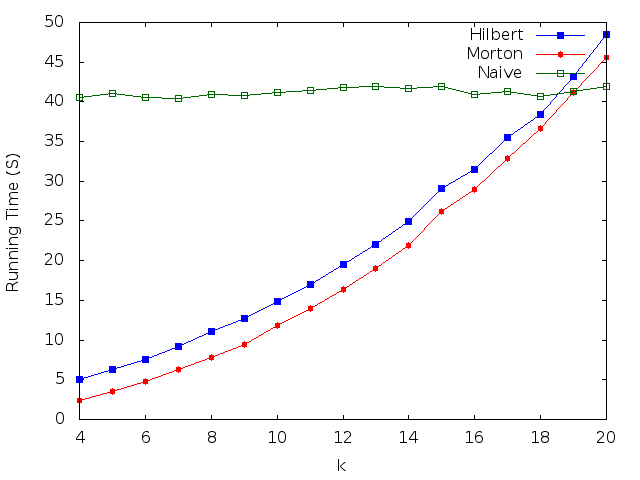
\includegraphics[scale=0.5]{YeaGra.png}
\caption{Running time analysis of the Yeast dataset ($d = 8$, $n = 1484$).}
\label{run-yeast}
\par\vspace{\intextsep}
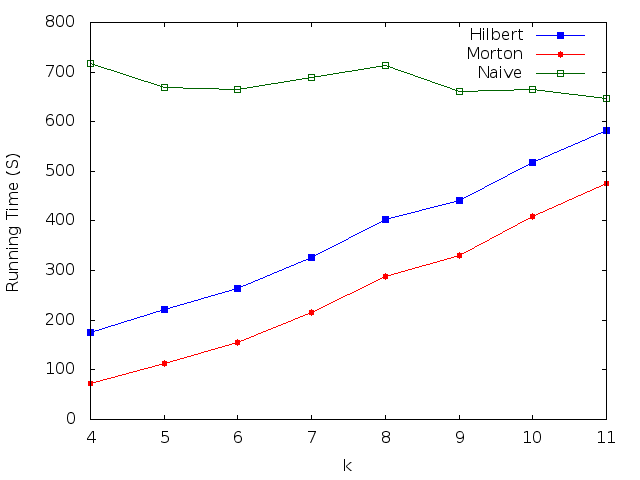
\includegraphics[scale=0.5]{ArcGra.png}
\caption{Running time analysis of the ARCENE dataset ($d = 1024$, $n = 700$).}
\label{run-arcene}
\end{center}
\end{figure}

\begin{figure}
\begin{center}
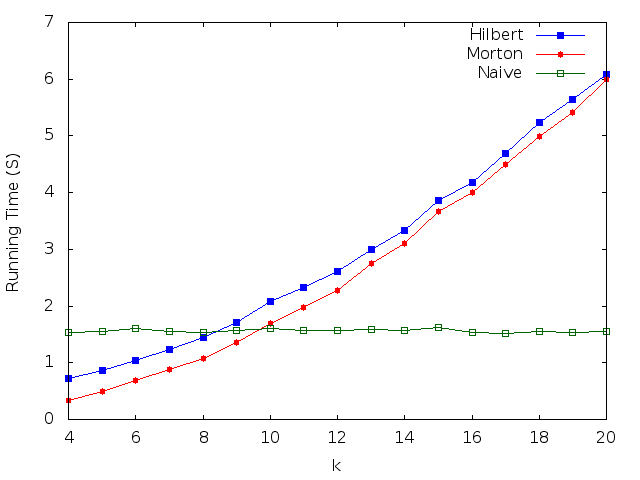
\includegraphics[scale=0.5]{LatGra.png}
\caption{Running time analysis of the integer lattice dataset ($d = 2$, $n = 1600$).}
\label{run-lattice}
\end{center}
\end{figure}

\begin{figure}
\begin{center}
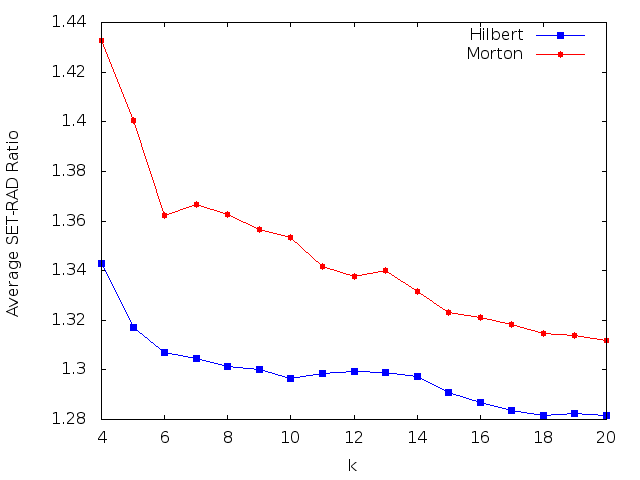
\includegraphics[scale=0.5]{YeaGra2.png}
\caption{Approximation bound of the Yeast dataset ($d = 8$, $n = 1484$).}
\label{approx-yeast}
\end{center}
\end{figure}

\begin{figure}
\begin{center}
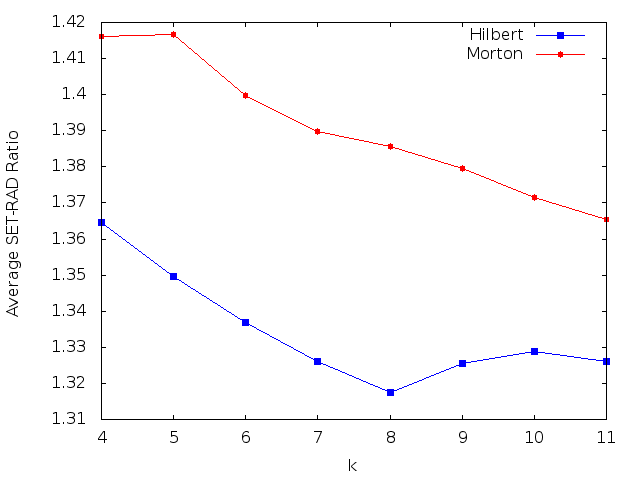
\includegraphics[scale=0.5]{ArcGra2.png}
\caption{Approximation bound of the ARCENE dataset ($d = 1024$, $n = 700$).}
\label{approx-acrene}
\end{center}
\end{figure}

\begin{figure}
\begin{center}
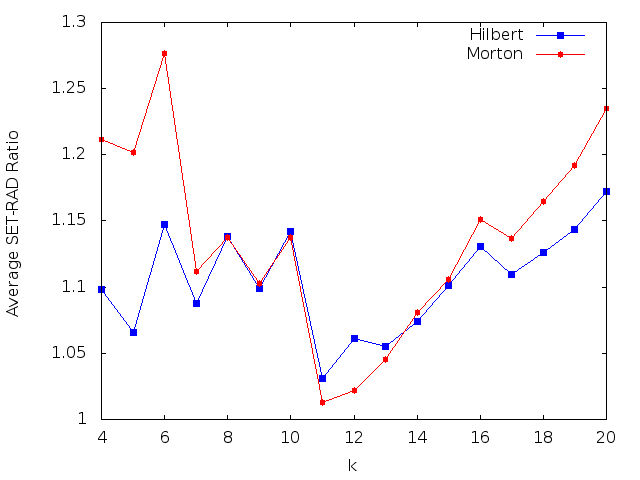
\includegraphics[scale=0.5]{LatGra2.png}
\caption{Approximation bound of the integer lattice dataset ($d = 2$, $n = 1600$).}
\label{approx-lattice}
\end{center}
\end{figure}

\bibliographystyle{amsplain}
\bibliography{mybiblio}

\end{document}

